\section{Projektplanung- und Management}\label{sec:section-one}

In diesem Kapitel wird in Abschnitt~\ref{subsec:subsection-one-one} zu Beginn der bisherige Stand aus dem ersten Praxismodul zusammengefasst.
Abschnitt~\ref{subsec:subsection-one-two} behandelt die Zielsetzung dieses zweiten Praxismoduls.
Die aktuelle Projektorganisation wird im dritten Abschnitt~\ref{subsec:subsection-one-three} definiert.
Abschnitt~\ref{subsec:subsection-one-four} gibt abschließend einen aktualisierten Überblick über die verwendeten Tools.

\subsection{Rückblick auf Praxismodul I}\label{subsec:subsection-one-one}

Das Praxismodul I begann mit der Projektidee und Motivation eine webbasierte Plattform, \textbf{\textit{Collectiqo}} genannt, zu erstellen um Sammlungen \textit{(eng. collections)} aller Art übersichtlich zu katalogisieren.
Innerhalb der Projektdokumentation umfassten zwei umfangreichere Kapitel die Projektplanung und das Projektmanagement.
Die Planung bestand aus den Abschnitten Zieldefinition, Teilergebnisse, Projektsteckbrief, Definitions of Done und Projektstrukturplan.
Das Projektmanagement behandelte die Abschnitte Organigramm, Ablaufplanung, Stakeholder- und Risikoanalyse, Kosten- und Aufwandsplanung, sowie verwendete Tools.

Das Projekt sollte mit frei zugänglicher Software und Tools basierend auf Education-Programmen realisiert werden.
Die Projektstruktur basierte auf einem Git Repository, Administration und Programmierung erfolgte mithilfe Webstorm, einer IDE der Firma JetBrains.
Anhand Docker Compose wurde eine dreigeteilte Containerisierung genutzt.
Container 1 stelle das Front- und Backend dar, die anderen beiden Container waren jeweils die Datenbanksysteme MySQL (User-Management) und mongoDB (Sammlungen).
Die Programmiersprache war JavaScript, das Frontend wurde mit HTML, CSS und EJS entwickelt, das Backend setzt auf Node.js, express und axios.

Zum Ende des Praxismoduls I wurde die Plattform in einer Präsentation u.\,a.\ Live vorgestellt und die Projektdokumentation abgegeben.
Viele grundlegende Ziele wurden erfolgreich abgeschlossen, darunter die grundlegende Implementierung Backend- und Frontend-Systeme.
Das Datenbanksystem wurde vollständig umgesetzt.
Die vollumfängliche Verknüpfung der Systeme war noch in Bearbeitung, insbesondere die Verbindung zwischen Frontend und Backend.
Account-Erstellung, Benutzer-Login und die Nutzung vorhandener Sammlungs-Templates funktionierten bereits.
Das Anlegen eigener Templates war im Backend implementiert, fehlte aber noch im Frontend.
Einfache Unit-Tests wurden erfolgreich implementiert.

Viele der geplanten Ziele wurden erreicht, dennoch traten einige Herausforderungen und Verzögerungen auf.
Das Team erwarb umfangreiche neue Kenntnisse in verschiedenen Bereichen, die Lernkurve war allerdings steiler als zuvor erwartet, was auf die Komplexität der Webentwicklung und neue Tools wie Docker bzw. das dokumentenorientierte NoSQL-Datenbankmanagementsystem MongoDB zurückzuführen war.
Vereinzelte Ziele mussten dadurch allerdings zeitlich verschoben werden oder waren zum Zeitpunkt der Abgabe des Praxismoduls I noch in Bearbeitung.
Das Projekt sollte daher im Praxismodul II fortgeführt werden.

\newpage

\subsection{Zielsetzungen im Praxismodul II}\label{subsec:subsection-one-two}

Das Praxismodul II baut auf den Ergebnissen des ersten Praxismoduls auf und setzt die Entwicklung der Plattform \textbf{\textit{Collectiqo}} fort.
Dies umfasst sowohl die Fertigstellung geplanter, aber noch nicht umgesetzter Funktionen als auch die Implementierung neuer Ideen.
Die Projektplanung und -organisation soll dabei deutlich kürzer gehalten werden, da diese bereits im ersten Praxismodul ausführlich behandelt wurde.
Hauptaugenmerk liegt daher auf der technischen Implementierung und der Erweiterung der Funktionalitäten.

Die Projektstruktur soll zu Beginn überarbeitet werden.
Eine Umstrukturierung des Git-Repositories ist geplant, um die Übersichtlichkeit zu verbessern, die Komplexität zu reduzieren und den Entwicklungsworkflow zu optimieren.
Die Dockerumgebung wird erweitert, indem Client- und Serverseite in separate Container aufgeteilt werden.
Fortan wird das Projekt aus mindestens vier Containern bestehen: Frontend (clientseitig), Backend (serverseitig) und den beiden Datenbanken für User bzw\. Sammlungen.

Eine umfangreichere Designanalyse soll durchgeführt werden.
Welche rechtlichen Vorgaben für den Betrieb einer Webseite zu beachten sind, soll dabei genauer untersucht und erläutert werden.
Derzeit noch fehlende Bausteine sollen somit ergänzt werden.
Im Frontend ist ein visuelles Redesign geplant.
Basierend auf den bereits erstellten HTML-Grundlagen soll ein einheitliches und modernes Erscheinungsbild entstehen.

Der Hauptfokus liegt auf der Erweiterung der Sammlungsverwaltung, insbesondere der Erstellung eigener Templates und dem Editieren bestehender Sammlungen.
Das Backend soll robuster gestaltet und die Verknüpfung mit dem Frontend vervollständigt werden.
Auf Datenbankebene ist die Absicherung durch Constraints vorgesehen, um die Datenintegrität zu gewährleisten.
Kleinere Bugs in Front- und Backend sollen behoben werden.


Für das Praxismodul II sollen ebenfalls Funktionserweiterung einfließen.
Ein wichtiger Schwerpunkt liegt auf der Erstellung von Integrationstests, die die bestehenden einfachen Unit-Tests ergänzen sollen.
% TODO: Sofern die Sharing Funktion verfolgt wird!
Als neue Funktion ist die Implementierung einer Sharing-Möglichkeit für Sammlungen vorgesehen.
Dieser Community-Aspekt erfordert auch einen Ausbau der Benutzereinstellungen.


\subsection{Projektorganisationen}\label{subsec:subsection-one-three}

Das Team besteht unverändert aus den vier Studierenden Anika, Darko, Lorenz und Robin.
Projektbetreuer ist dankenswerterweise weiterhin Herr Prof.\, Dr.\, Dirk Schweim.
Durch die im ersten Praxismodul gewonnenen Erfahrungen in Bezug auf Umfang und Komplexität einzelner Aufgaben wurde die Rollen- und Aufgabenverteilung innerhalb des Teams leicht angepasst.
Die Organisation und Übersicht der einzelnen Aufgaben wird weiterhin mit einem Projektmanagementprogramm gesteuert, wöchentliche Meetings dienen der Abstimmung und dem Austausch.

Anika und Darko sind für die grafische und technische Frontendentwicklung zuständig, wobei Anika sich auf die grafische Entwicklung basierend auf dem Design konzentriert und Darko die technische Umsetzung in JavaScript übernimmt.
Für die Backend-Entwicklung ist Lorenz zuständig, er übernimmt ebenfalls die Integrationstests.
Um die Datenbanksysteme und Docker kümmert sich Robin, des Weiteren übernimmt er den Lead für die Dokumentation sowie Präsentation.
Da Lorenz sich in Praxismodul I bereits intensiv mit Docker auseinandergesetzt hat, wird er Robin hier unterstützen.


\subsection{Verwendete Tools}\label{subsec:subsection-one-four}

Der überwiegende Teil der im Projekt verwendeten Tools ist unverändert geblieben.
Es soll nur auf einige wenige Änderungen eingegangen werden, die sich im Vergleich zum ersten Praxismodul ergeben haben.

In der Kategorie \textit{Allgemein} ist Google Forms, das für die Umfrage im Praxismodul I genutzt wurde, weggefallen.
Hinzugekommen ist die Nutzung von Photoshop, welches über vergünstigte Bildungskonditionen bezogen wurde.
Es dient der Erstellung von Grafiken für die Plattform sowie in der Designanalyse und der Erstellung von Mockups.
Das Projektmanagementtool YouTrack wurde durch ein übersichtlicheres und in der Industrie verbreiteteres Tool ersetzt.
Jira wird fortan in der Free-Version genutzt, die bis zu 10 Nutzer kostenlos und für die Vorhaben ausreichend ist.
Zugriff und Verwaltung erfolgt über die Atlassian Cloud mithilfe der Browseroberfläche und den mobilen Apps.

Im Bereich \textit{Backend} ist axios weggefallen, da es im ersten Praxismodul nur für die Anbindung an die REST-API genutzt wurde.
Da die REST-API im Backend selbst implementiert wird, ist axios nicht mehr notwendig. %TODO: Stimmt das technisch so?^^

Nachfolgend wird eine Übersicht der verwendeten Tools als Grafik gegeben, die im Praxismodul II zum Einsatz kommen.
Die Aufteilung des Frontends und Backends in separate Container wird ebenfalls dargestellt.

\begin{figure}[H]
    \centering
    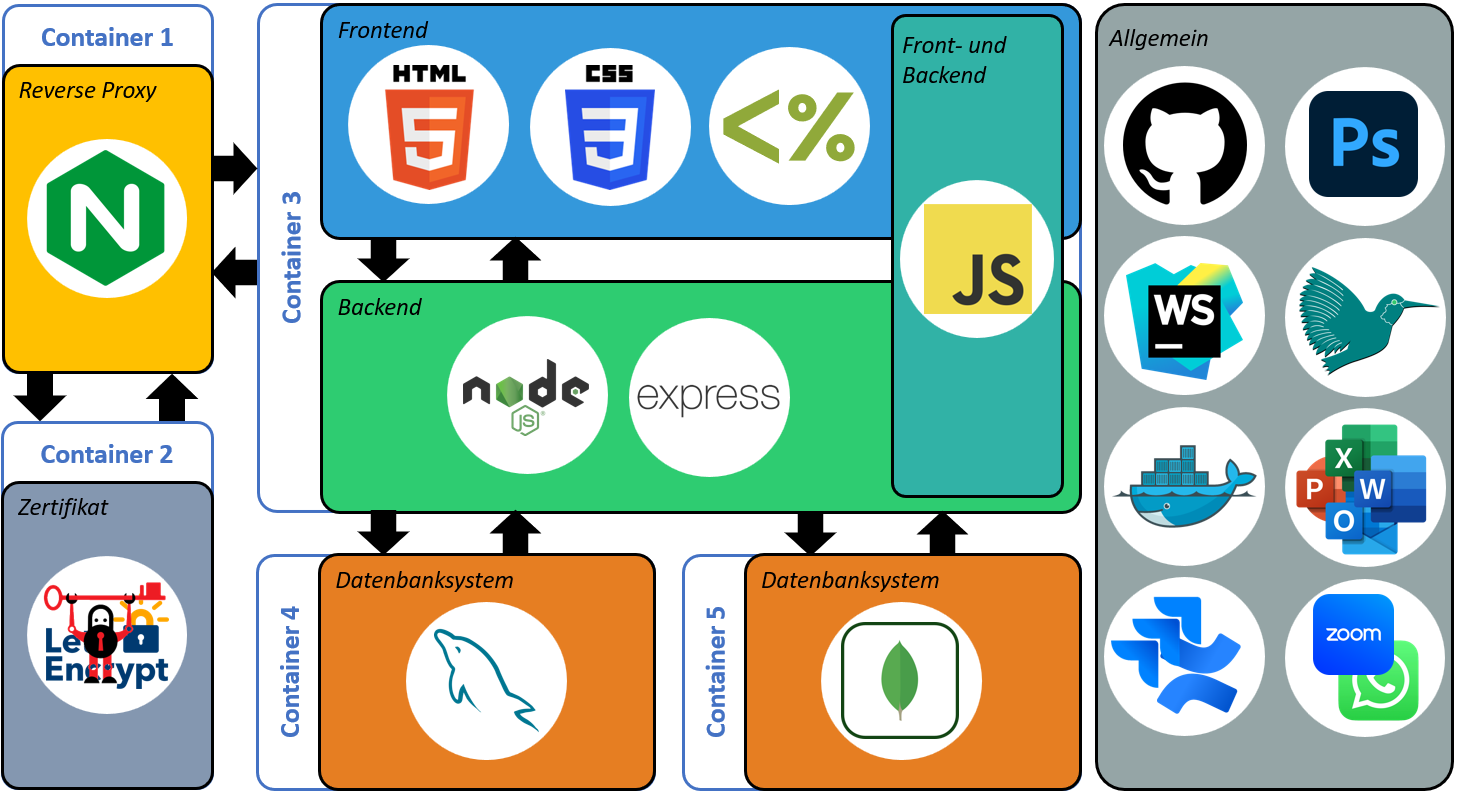
\includegraphics[width=1.0\textwidth]{tools}
    \caption{Übersicht der Tools}\label{fig:uebersicht-tools}
\end{figure}


